\section{Bitcoin}\label{sec:Bitcoin}
%%%%%%%%%%%%%%%%%%%%%%%%%%%
% *** FIRST SUB-SECTION ***
%%%%%%%%%%%%%%%%%%%%%%%%%%%
\subsection{Introduction}

Bitcoin it's the first fully decentralized cryptocurrency. It was invented by
Satoshi Nakamoto in 2008 and it was the first real implementation of Blockchain.
Bitcoin can be either defined as a protocol, a digital currency and a platform.

Bitcoin can be seen as a combination of
\vspace{-\topsep}
\begin{itemize}
  \item[-] a decentralized peer-to-peer-network (the Bitcoin protocol)
  \item[-] a public transaction ledger (the blockchain)
  \item[-] a set of rules for validating transactions (consensus rules)
  \item[-] a mechanism for reaching distributed consensus on the blockchain (distributed
  consensus algorithm)
\end{itemize}
\vspace{-\topsep}
that allows the usage of the digital currency named bitcoin.

From now on, Bitcoin with the capital $B$ will refer to the Bitcoin protocol
while bitcoin with the lowercase $b$ will refer to the bitcoin currency.



Bitcoin is a distributed peer-to-peer system in which users can exchange
currency over the network just as it can be done with conventional currency.
However, unlike traditional currencies, bitcoins are entirely virtual and thus
there are no physical coins. In particular, there are not even virtual coins since
they are implied in the transactions that send value from a sender to a receiver:
users have private keys which allow them to prove the ownership of bitcoins and
sign transactions in order to unlock the value and transfer it to another user.
These keys are the only requirement for spending bitcoins and therefore they are
protected in wallets stored in the user's devices.

\subsubsection*{The reference implementation}
Bitcoin is an open source project and is developed by a community of volunteers.
The first implementation was released by Satoshi Nakamoto in 2008 (the only member
of the development community at the time). That implementation during the years
has been heavily modified and improved evolving into what is known as \emph{Bitcoin
Core}, which is now the reference implementation of the Bitcoin system. This
implementation is considered the authoritative one and it specifies how each
part of the system has to be implemented.










%%%%%%%%%%%%%%%%%%%%%%%%%%%
% *** THIRD SUB-SECTION ***
%%%%%%%%%%%%%%%%%%%%%%%%%%%
\subsection{Scripts} \label{sec:scripts}Bitcoin uses a simple stack-based
programming language called ``Script'' for describing how bitcoins can be spent
and transferred in order to extend flexibility and support different types of
transactions. Essentially, a Bitcoin script is a list of instructions recorded
with each transaction that describes how the next person wanting to spend the
Bitcoins being transferred can gain access to them \cite{script-bitcoin-wiki}.

Script is a very simple language and it's not Turing complete. The language has
been deliberately designed limiting its operators (it doesn't have loop
operators and complex control flow different than conditional control flow) in
order to avoid abuses of the scripts for conducting denial of service attacks,
since the transaction scripts have to be executed on each node of the network.

Script supports a number of functions called ``Opcodes'', uses a reverse polish
notation in which every operand is followed by its operators and it's evaluated
from the left to the right using a LIFO stack. Table \ref{tab:opcode-example} shows the most common
Opcodes while figure \ref{fig:script-example} shows an example of Script program.



\begin{table}[!ht]
\footnotesize
\begin{tabularx}{\textwidth}{l X}
\hline
\textbf{Opcode} & \textbf{Description}  \\\hline
OP\_CHECKSIG & This takes a public key and signature and validates the signature of the hash of the transaction. If it matches, then TRUE is pushed onto the stack; otherwise, FALSE is pushed.  \\
\\
OP\_EQUAL & This returns 1 if the inputs are exactly equal; otherwise, 0 is returned.  \\
\\
OP\_DUP & This duplicates the top item in the stack.  \\
\\
OP\_HASH160 & The input is hashed twice, first with SHA-256 and then with RIPEMD-160. \\
\\
OP\_VERIFY & This marks the transaction as invalid if the top stack value is not true. \\
\\
OP\_EQUALVERIFY & This is the same as OP\_EQUAL, but it runs OP\_VERIFY afterwards. \\
\\
OP\_CHECKMULTISIG & This takes the first signature and compares it against each public key until a match is found and repeats this process until all signatures are checked. If all signatures turn out to be valid, then a value of 1 is returned as a result; otherwise, 0 is returned. \\
\hline
\end{tabularx}
\caption{\footnotesize Most commonly used Opcodes. Taken from the
bitcoin developer's guide \cite{bitcoin-developer-guide}. }
\label{tab:opcode-example}
\end{table}








%%%%%%%%%%%%%%%%%%%%%%%%%%%
% *** THIRD SUB-SECTION ***
%%%%%%%%%%%%%%%%%%%%%%%%%%%
\subsection{Keys and Addresses}
As mentioned in this chapter's introduction, ownership of bitcoin is established
through digital keys, bitcoin addresses, and digital signatures.

In order to be included in the Bitcoin blockchain, transactions require a valid
signature which can be generated only with a private (secret) key. The private
key, therefore, proves the ownership of bitcoins by signing transactions and
transferring value from a user to another. Keys come in pairs consisting of a
private (secret) key and a public key and they are generated through Elliptic
Curve Cryptography. In analogy with the traditional banking, the public key can
be seen as the bank account number while the private key as the secret PIN (or
the signature on a check) which provides control over the account by allowing to
unlock the value and transferring it to other people.

\subsubsection{Adresses} An address is a unique string of digits and characters
which identify the originator and/or the destination of a transaction. Addresses
are derived from public keys through one-way cryptographic hashing in order to
obtain the public key fingerprint. In particular, a Bitcoin address is derived
by hashing the user's public key it twice, first with the SHA-256 algorithm and
then with RIPEMD160. This produces a 160-bit hash, which is then prefixed with a
version number and finally encoded using Base58Check encoding. The final result
is a 26-35 characters string which begins with ``$1$'' (public key address) or
``$3$'' (pay-to-script-hash address) and it looks like the the string below:
\begin{center} \code{1J7mdg5rbQyUHENYdx39WVWK7fsLpEoXZy} \end{center} The
generation process scheme is shown in figure \ref{fig:address-generation}.

\begin{figure}[!htb]
	\centering
	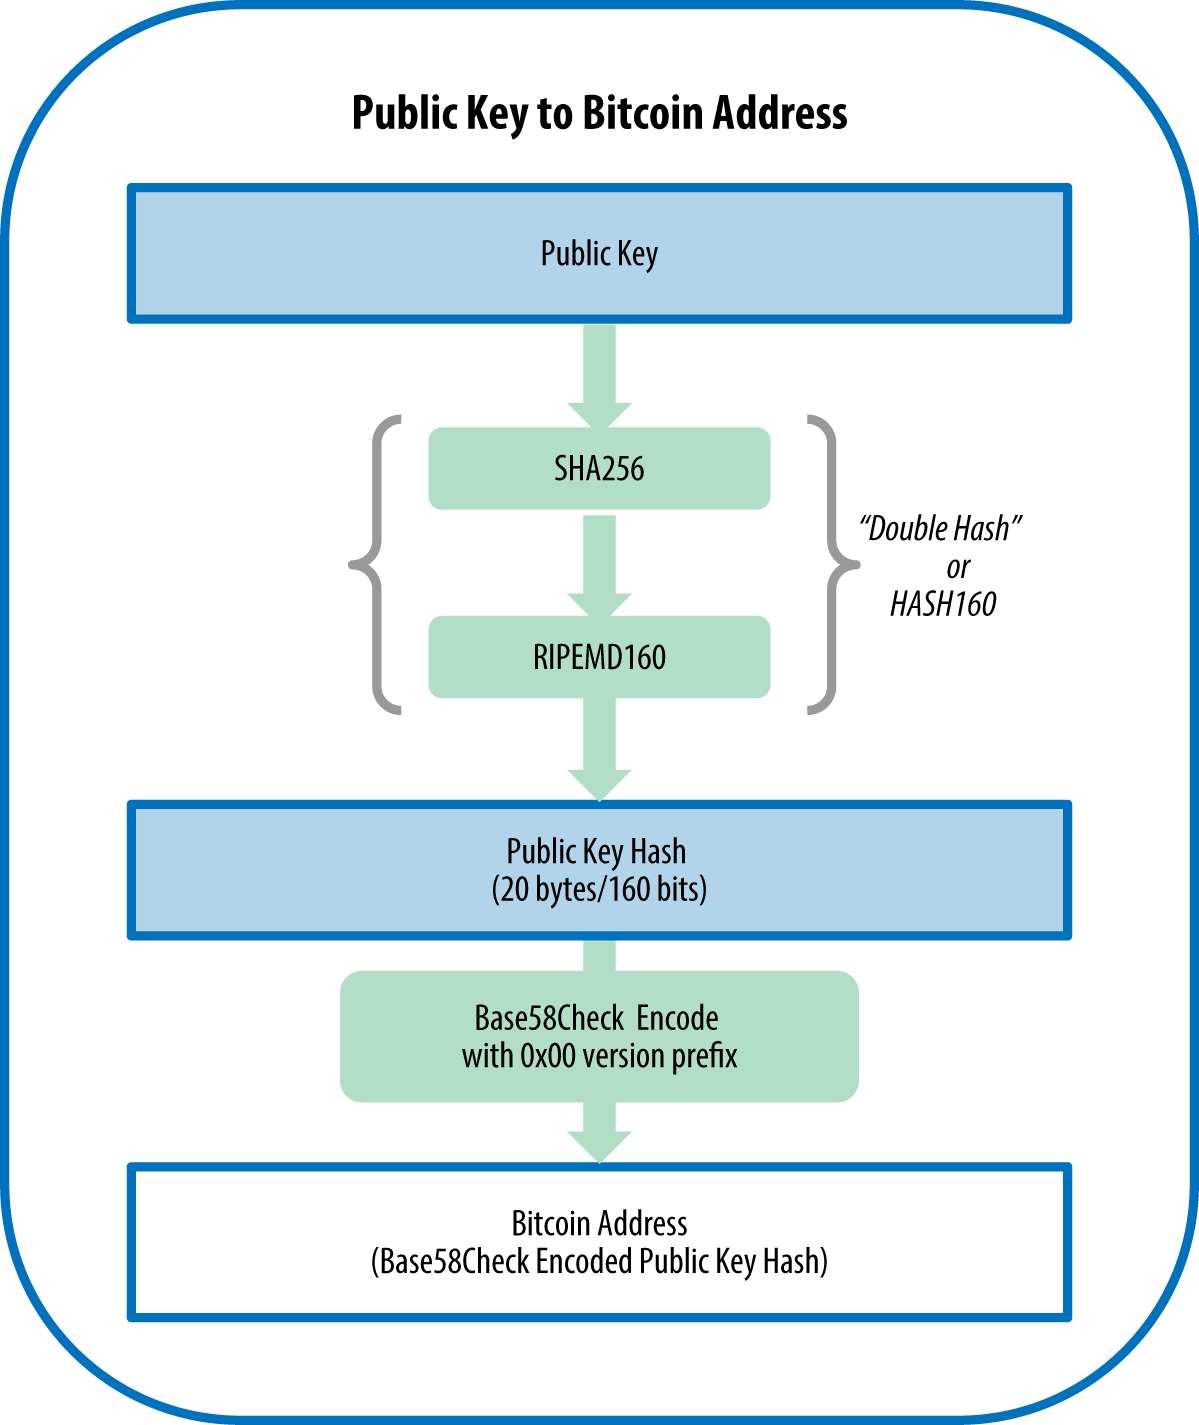
\includegraphics[width=0.85\linewidth]{img/address-generation.png}
	\caption{Bitcoin address generation scheme}
	\label{fig:address-generation}
\end{figure}

\paragraph{Base58 and Base58Check} Base58 is an encoding scheme which allows to
represent long numbers as alphanumeric strings. It is a subset of Base64, which
represent numbers using 26 lowercase letters, 26 capital letters, 10 numerals,
and 2 more ``special'' characters and it's usually used to encode email
attachments. In particular, Base58 is Base64 without all that characters that
are frequently mistaken for one another, namely it is Base64 without the 0
(number zero), O (capital o), l (lower L), I (capital i) and the two special
characters. Base58Check is a Base58 encoding with an additional checksum of four
bytes added to the end of the data that is being encoded which prevents a
mistyped bitcoin address from being accepted by the wallet software as a valid
destination.


\paragraph{P2SH and P2PKH}  As already mentioned before, Bitcoin addresses that
begin with the number ``$3$'' are pay-to-script hash (P2SH) addresses. Unlike
the address which starts with ``$1$'', also known as pay-to-public-key-hash
(P2PKH), which are associated with a public key owned by a user, the P2SH
addresses designate the beneficiary of a Bitcoin transaction as the hash of a
script. When a user sends a bitcoin to a P2PKH address, that bitcoin can only
be spent by the receiver by presenting the corresponding private key signature
and public key hash associated with its address. When instead the bitcoin is sent to
a P2SH address, namely to the hash of a script, the requirements for spending that
bitcoin are defined by the script and are usually more restrictive (for example it
could be required more than one signature to prove the ownership). A P2SH address
is derived from a transaction script in the same way a P2PKH address is derived
from a public key (double hashing + Base58Check encoding).


\subsubsection{Keys}
Public and private keys in Bitcoin are generated through ECC and they can be
represented in different formats. All the possible representations, even if they
look different, correspond to the same number. This has been done in order to
facilitate people to read and transcribe the keys without introducing errors.

\paragraph{Private keys}
Private keys are simply a 256-bit random number. For generating it, Bitcoin
software uses the underlying operating system’s random number generators which
usually is initialized by a human source of randomness, like for example the elapsed
time between the pressure of the keys of the keyboard.

\paragraph{Private key formats}
The private key can be represented in different formats (shown in table
\ref{tab:private-key-formats}), each one corresponding to the same 256-bit number.
Different formats are used in different circumstances: for example Hexadecimal
and raw binary formats are used internally in software while WIF is used by users.
\begin{table}[h!]
\centering
\resizebox{\textwidth}{!}{%
\begin{tabular}{@{}lll@{}}
\toprule
\multicolumn{1}{c}{\textbf{Type}} & \multicolumn{1}{c}{\textbf{Prefix}} & \multicolumn{1}{c}{\textbf{Description}}                                     \\ \midrule
Raw                               & None                                & 32 bytes                                                                     \\
Hex                               & None                                & 64 hexadecimal digits                                                        \\
WIF                               & 5                                   & Base58Check encoding \\
WIF-compressed                    & K or L                              & As above, with added suffix 0x01 before encoding                             \\ \bottomrule
\end{tabular}%
}
\caption{Private key representation formats \cite{antonopoulos2017mastering}}
\label{tab:private-key-formats}
\end{table}

\paragraph{Public key generation}
Public keys are generated starting from the private keys using elliptic curve
multiplication, which is a so-called ``trap door'' function: it is easy to do in
one direction (multiplication) and impossible to do in the reverse direction (division).
Bitcoin uses the elliptic curve and the set of constants specified by the secp256k1
standard, defined by the NIST. The elliptic curve used is defined by the following
equation:
\begin{equation}\label{eq:bitcoin-curve}
  y^2 = (x^3 + 7)~\text{over}~(\mathbb{F}_p)
\end{equation}
\begin{center}
  or, equivalently:
\end{center}
\begin{equation}
  y^2 \bmod p = (x^3 + 7) \bmod p
\end{equation}
where $p = 2^{256} – 2^{32} – 2^9 – 2^8 – 2^7 – 2^6 – 2^4 – 1$ is a very large prime number.
Starting from the private key $k$, the public key $K$ is calculated by multiplying
it by a predetermined point on the curve called the generator point $G$ (defined
by the secp256k1 standard) in order to produce another point somewhere else on
the curve, which will correspond to the public key $K$:
\[K = k * G\]
Since the generator point $G$ is always the same for all bitcoin users, a
private key $k$ multiplied with $G$ will always result in the same public key $K$.
The relationship between $k$ and $K$ is fixed and known but it can only be
calculated in one direction (from $k$ to $K$), so it's impossible to derive from
an address (derived from K) the corresponding user's private key.

\paragraph{Public key formats} In Bitcoin, since ECC is used, a public key in
the uncompressed format is a point on an elliptic curve consisting of the
coordinates pair $(x,y)$. Uncompressed public keys are presented with the prefix
\code{04} followed by two 256-bit numbers, one for each coordinate, and
therefore they are 65 Bytes long. The compressed format instead includes only
the x-coordiante since the y one can be derived from it and by solving the
equation \eqref{eq:bitcoin-curve} it uses the prefixes \code{03}, if the
y-coordinate is an odd number, or \code{02}, if it is an even number. The length
of a compressed public key is therefore 33 Bytes. Compressed public keys were
introduced in order to reduce the size of the transactions, since the most of
them also include the public key. The reason why two different prefixes are
required for compressed keys is that the left side of the equation
\eqref{eq:bitcoin-curve} is $y^2$ and therefore the solution for $y$ is a square
root, which can have a ``positive'' or ``negative value'': graphically, this
means that the y-coordiante can either be above or below the x-axis and
therefore two different points can be identified since the curve is symmetric.
Actually since we are in fhe field $\mathbb{F}_p$ it doesn't make sense talking
about positive and negative values: the y-coordinate can, in fact, be
\emph{even} or \emph{odd} (which correspond to the positive/negative terms used
before).

Note that a public key in both compressed and uncompressed formats always
corresponds to the same private key, even if the two formats have a different
representation. The address derived from the compressed public key however is
different from the address derived from the uncompressed one. To solve this
issue, compressed private keys have been introduced: a compressed private key is
a ``private key from which only compressed public keys should be derived'',
while uncompressed private keys are ``private keys from which only uncompressed
public keys should be derived'' \cite{antonopoulos2017mastering}.











%%%%%%%%%%%%%%%%%%%%%%%%%%%
% *** FOURTH SUB-SECTION ***
%%%%%%%%%%%%%%%%%%%%%%%%%%%
\subsection{Transactions}\label{sec:transactions} Transactions are data structures that encode the
transfer of value between participants in the bitcoin system. In important to
point out that they are not encrypted and are publicly visible in the
blockchain. Blockchain blocks are made up of transactions and these can be
viewed using any online blockchain explorer.

\subsubsection{Transaction inputs and outputs}
A transaction includes at least one input and output: inputs can be seen as
coins being spent that the user has created in a previous transaction while
outputs as coins being created.

\paragraph{Outputs and UXTO} In particular, outputs are discrete and indivisible
units of bitcoin measured in \emph{Satoshi}\footnote{One Satoshi
$=10^{-8}$bitcoins}, recorded on the blockchain and recognized as valid by the
network. All the available and spendable outpus are stored in the blockchain and
they are called \emph{unspent transaction outputs} or \emph{UTXO}. The balance
shown by Wallets application is nothing more than the aggregated value all the
UTXOs the user can spend with the keys it controls. Note that a UXTO can only be
spent in its entirety by a transaction, consequently, if an UTXO is larger than
the desired value of a transaction, it must still be consumed in its entirety
and change must be generated in the transaction (most of the bitcoin
transactions generate change). Transaction outputs consist of two parts: an
amount of bitcoin (expressed in Satoshis) and a cryptographic puzzle that
determines the conditions required to spend the output. This puzzle is also
known as a \emph{locking script} and it consists of a digital signature and
public key proving the ownership of the UXTO.

\paragraph{Inputs} Transaction inputs consist of which UTXO will be consumed
(can be more than one single UXTO) and a proof of ownership through the
unlocking script to unlock the selected UXTO.


\subsubsection{Transactions structure}

\begin{table}[h!]
\centering
\resizebox{\textwidth}{!}{%
\begin{tabularx}{\textwidth}{l l X}
\toprule
\textbf{Field} & \textbf{Size} & \textbf{Description}                                    \\ \midrule
Version Number                    & 4 bytes                             & Used to specify rules to be used by the miners and nodes for transaction processing.                                                                     \\
\\
Input counter                     & 1-9 bytes                           & The number of inputs included in the transaction.                                                       \\
\\
List of inputs                    & variable                            & Each input is composed of several fields, including Previous transaction hash, Previous Txout-index, Txin-script length, Txin-script, and optional sequence number. The first transaction in a block is also called a coinbase transaction. It specifies one or more transaction inputs. \\
\\
Output counter                    & 1-9 bytes                           & A positive integer representing the number of outputs.                        \\
\\
List of Outputs                   & variable                            & Outputs included in the transaction. \\
\\
lock\_time                         & 4 bytes                             & This defines the earliest time when a transaction becomes valid. It is either a Unix timestamp or a block number.                             \\ \bottomrule
\end{tabularx}
}
\caption{Structure of Bitcoin transactions}
\label{tab:transaction-structure}
\end{table}


\subsubsection{Transactions life cycle}
This is the typical life cycle of a transaction:
\begin{enumerate}
  \item A sender sends a transaction (using a wallet application)
  \item The wallet signs the transaction using the sender's private key in order
  to prove the ownership of the value being transferred
  \item The transaction is broadcasted to the Bitcoin network using a flooding algorithm.
  \item Mining nodes include this transaction in the next block to be mined.
  \item Once a mining node solves the Proof of Work problem it broadcasts the
  newly mined block to the network and the confirmation process starts: each
  nodes verify the block and propagate it further
  \item The receiver start to receive confirmations. After approximately six
  confirmations, the transaction is considered finalized and confirmed.
\end{enumerate}




\subsubsection{Transaction fees} Most transactions include transaction fees.
These fees have to purposes: compensate the bitcoin miners and act as a security
mechanism by making economically infeasible for attackers to flood the network
with transactions. The value of the fees depends on the size of the
transaction since it's calculated by subtracting the sum of the outputs to the
sum of the inputs: \[Fees = Sum(Inputs) – Sum(Outputs)\] Fees also  act as an
incentive for miners to encourage them to include a user transaction in the
block the miners are creating. Each miner chooses from a memory pool which
transactions include in the block he will propose based on their priority:  a
transaction with a higher fee will be picked up sooner by the miners since it's
more profitable.


\subsubsection{Coinbase transactions} A particular kind of transaction is the
\emph{coinbase transaction}, which is created by the ``winning'' a miner and is
the first transaction in a block. This transactions create brand-new bitcoins
that the miner can spend as a reward for mining and do not consume UTXO,
instead, they have a special type of input called the \emph{coinbase}.








%%%%%%%%%%%%%%%%%%%%%%%%%%%
% *** FIFTH SUB-SECTION ***
%%%%%%%%%%%%%%%%%%%%%%%%%%%
\subsection{Wallets} A Wallet can be seen as an application that serves as a
user interface and manages user's money. Technically, however, a walles is a
data structure that securely stores the user's private keys required for
spending the bitcoins he possesses. A wallet, therefore, doesn't store ``money''
but only pairs of public/private keys that the user can use to sign transactions
and prove that he owns the coins, which are stored in the Blockchain as
transaction outputs.

There are two main kinds of wallet: \emph{deterministic} and
\emph{nondeterministic} wallets.

\paragraph{Nondeterministic wallets} In nondeterministic wallets each key is
independently generated starting from a random number, so the keys the wallet
stores are not related to each other. The main disadvantage of this kind of
wallets if that they are cumbersome to manage because each key has to be backed
up frequently (otherwise if the wallet becomes inaccessible then the founds
controlled by the key are irrevocably lost). This becomes quite a big problem
when dealing with avoidance of address reuse for enhancing privacy, which
consists of using each address for only one transaction (see section \ref{}):
each address corresponds to a private key, thus avoiding address reuse means
managing many keys that has to be backed up frequently. The Bitcoin core client
includes a type-0 nondeterministic wallet, which use for anything other than
simple tests is however discouraged by the developers.
\begin{figure}[!htb]
	\centering
	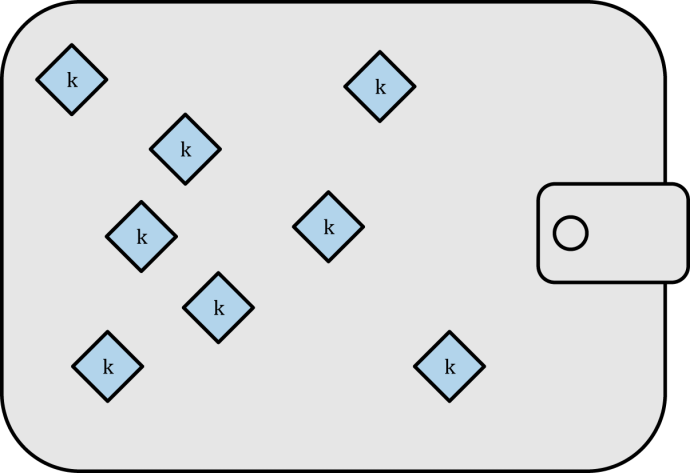
\includegraphics[width=0.5\linewidth]{img/nondeterministic-wallet.png}
	\caption{Type-0 nondeterministic wallet: a collection of randomly generated keys}
	\label{fig:nondeterministic-wallet}
\end{figure}

\paragraph{Deterministic wallets} In deterministic wallets all the keys are
derived from a single master key called the \emph{seed}, so all the keys are
related to each other and can be generated again if one has the original seed.
This means that a single backup of the seed at creation time is enough and thus
the wallet is easily manageable even if avoiding address reuse. The seed also
allows export/import a wallet, making therefore easy the migration of the user's
keys between different wallet implementations. The most advanced deterministic
wallet is the HD wallet defined by the BIP-32 standard, in which the keys are
derived in a tree structure such that a parent key can derive a sequence of
children keys, each of which can derive a sequence of grandchildren keys and so
on. Deriving keys in this ways offers two main advantages:
\begin{enumerate}
  \item The tree scheme offers great flexibility, for example a branch can be used
  for receiving payments while another one can be used for receiving only
  the change from outgoing payments. Moreover, in an enterprise context, different
  branches can be assigned to different departement of the company.
  \item The user can derive a sequence of public keys without the need to access
  the corresponding private keys. This is useful for example for making an insecure
  server issuing a different public key for each transaction without providing
  it the corresponding private keys so that it cannot spend the funds.
\end{enumerate}
Usually, the seeds are created according to the standard BIP-39, which defines
the seeds as a sequence of English words called \emph{mnemonic} so that they are
easy to transcribe, export and import across wallets. Today this standard is adopted
by the most of wallet implementations. \emph{The seed (and the mnemonic as well) has,
of course, to be random}. Below there's an example of comparison between a
hexadecimal seed and a mnemonic seed:
\begin{lstlisting}[title=Hex seed for a deterministic wallet:]
0C1E24E5917779D297E14D45F14E1A1A
\end{lstlisting}
\begin{lstlisting}[title=12-word mnemonic seed for a deterministic wallet:]
army van defense carry jealous true
garbage claim echo media make crunch
\end{lstlisting}

\begin{figure}[!htb]
	\centering
	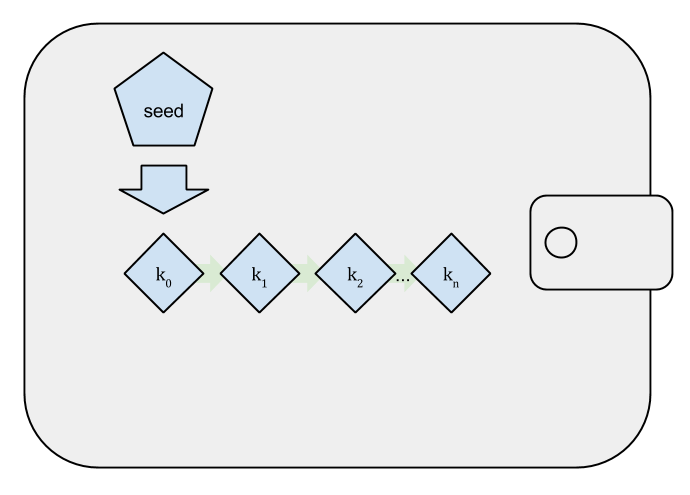
\includegraphics[width=0.5\linewidth]{img/deterministic-wallet.png}
	\caption{Type-0 nondeterministic wallet: a collection of randomly generated keys}
	\label{fig:deterministic-wallet}
\end{figure}


Bitcoin wallets can also be divided in other four categories:
\begin{enumerate}
  \item Mobile wallets: they are implemented using SPV (simple payment verification)
  nodes which allows power and storage constrained devices to verify transactions
  without downloading the whole blockchain.
  \item Desktop wallets: wallets that offer more services than mobile wallets,
  such as transactions anonymization and multisignature. They also generally
  support SPV mode.
  \item Online wallets: web-based wallets that store the keys in the cloud, providing
  high availability and ubiquity (they can be accessed from anywhere and from
  any device). The main issue is that the private keys are not under the control
  of the owner, which puts the BTCs that one possesses at serious risk.
  \item Hardware wallets: dedicated physical devices that hold private keys
  and offer payment assistance. They offer great security, but on the other hand,
  the main issue is the recoverability of the keys in case of hardware failure.
  An example of a hardware wallet is the Trezor hardware wallet \cite{trezorwallet}.
\end{enumerate}





%%%%%%%%%%%%%%%%%%%%%%%%%%%
% *** SIXTH SUB-SECTION ***
%%%%%%%%%%%%%%%%%%%%%%%%%%%
\subsection{The Bitcoin Blockchain} The Bitcoin blockchain is a linked list of
blocks of transactions, each one  identified by a SHA-256 hash. Each block
references the previous one (the \emph{parent block}) by embedding its hash in
the header. This chain of hashes goes back all the way to the first block ever
created, known as the \emph{genesis block}.

Although a block can have only one single parent, it can temporarily have
multiple children. This happens during a \emph{blockchain fork}, a temporary
situation which occurs when miners solve the proof of work of their block almost
simultaneously. Eventually, however, the forks are resolved and  only one child
block becomes part of the blockchain.

Modifying a block causes its hash to change. Consequently, since each block
contains in its header the hash of its parent block, changing a block causes
the child’s hash to change, which also requires a change in its child block hash
and so on. This cascade effect ensures that once a block has many generations
following it, it cannot be changed without forcing a recalculation of all
subsequent blocks: since this recalculation requires a huge computation, the
blockchain history is pratically immutable. This is a key feature of the Bitcoin
security.

\begin{figure}[!htb]
	\centering
	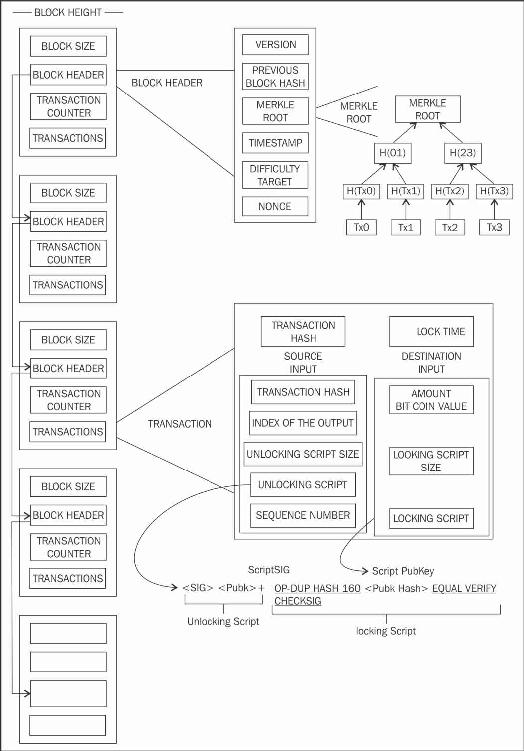
\includegraphics[width=0.9\linewidth]{img/bitcoin-blockchain-scheme.png}
	\caption{Bitcoin blockchain structure scheme}
	\label{fig:bitcoin-blockchain}
\end{figure}


\subsubsection{The block structure} Table \ref{tab:block-structure} summarize
the structure of a block of the blockchain, while table
\ref{tab:block-header-structure} shows the structure of the block header.

\begin{table}[h!]
\centering
\resizebox{\textwidth}{!}{%
\begin{tabularx}{\textwidth}{l l X}
\toprule
\textbf{Field} & \textbf{Size} & \textbf{Description}     \\ \midrule
Block size  & 4 bytes  & The size of the block, in bytes.       \\
\\
Block header & 80 bytes & Several fields form the block header. \\
\\
Transactions counter & 1-9 bytes & How many transactions the block contains. \\
\\
Transactions & Variable & The transactions recorded in the block \\ \bottomrule
\end{tabularx}
}
\caption{Structure of a Bitcoin block}
\label{tab:block-structure}
\end{table}



\begin{table}[h!]
\centering
\resizebox{\textwidth}{!}{%
\begin{tabularx}{\textwidth}{l l X}
\toprule
\textbf{Field} & \textbf{Size} & \textbf{Description}     \\ \midrule
Version  & 4 bytes  & A version number to track software/protocol upgrades.       \\
\\
Previous block hash  & 32 bytes & A reference to the hash of the previous (parent) block in the chain. \\
\\
Merkle root & 32 bytes & A hash of the root of the Merkle tree of this block’s transactions. \\
\\
Timestamp & 4 bytes & The approximate creation time of this block (seconds from Unix Epoch). \\
\\
Difficulty target & 4 bytes & The Proof-of-Work algorithm difficulty target for this block. \\
\\
Nonce & 4 bytes & A counter used for the Proof-of-Work algorithm. \\ \bottomrule
\end{tabularx}
}
\caption{Structure of a Bitcoin block header}
\label{tab:block-header-structure}
\end{table}


\subsubsection{Merkle trees}\label{sec:Merkle-trees} Each block summmarize all the transactions it
contains using a Merkle tree, which is a data structure used for efficiently
summarizing and verifying the integrity of large sets of data. A Merkle tree  is
a binary tree containing hashes and it produces an overall digital fingerprint
of the entire set of transactions, providing a very efficient method to verify
whether a transaction is included in a block. The hash algorithm used in
bitcoin’s Merkle trees is double-SHA256 (SHA256 applied twice).

In the Bitcoin blocks headers only the 32-byte hash corresponding to the tree
root is stored, which summarizes all the transactions and allows a node to check
whether a specific transaction is included in the block by computing the
$log_2(N)$ hashes which make up a \emph{Merkle path} connecting the transaction
to the root of the tree, with $N$ number of transactions of the block. Figure
\ref{fig:Merkle-tree-path} shows an example of Merkle path, while table
\ref{tab:Merkle-tree-sizes} compares the size of a block to the size of a Merkle
path.

 Thanks to Merkle trees, a node can download just the block headers (80 bytes
 per block) and still be able to verify whether a transaction is included in a
 block by retrieving a small Merkle path from a full node (which stores the
 complete blockchain) instead of storing or retrieving the full block, which is
 a lot more efficient as pointed out in table \ref{tab:Merkle-tree-sizes}.

 The nodes that do not maintain a full copy of the blockchain are \emph{called
 simplified payment verification} (SPV) nodes and they use Merkle paths to
 verify transactions without downloading full blocks.

 \begin{table}[h!]
 \footnotesize

 \centering
 \resizebox{\textwidth}{!}{%
 \begin{tabularx}{\textwidth}{l l l l}
 \toprule
 \textbf{Number of transactions}	& \textbf{Approx size of block} & \textbf{Path size} &	\textbf{Path size}   \\ \midrule
 16 transactions & 4 kilobytes & 4 hashes & 128 bytes \\
 \\
 512 transactions & 128 kilobytes & 9 hashes & 288 bytes \\
 \\
 2048 transactions & 512 kilobytes & 11 hashes & 352 bytes \\
 \\
 65535 transactions & 16 megabytes & 16 hashes & 512 bytes \\
 \bottomrule
 \end{tabularx}
 }
 \caption{Merkle tree efficiency}
 \label{tab:Merkle-tree-sizes}
 \end{table}


\begin{figure}[!htb]
	\centering
	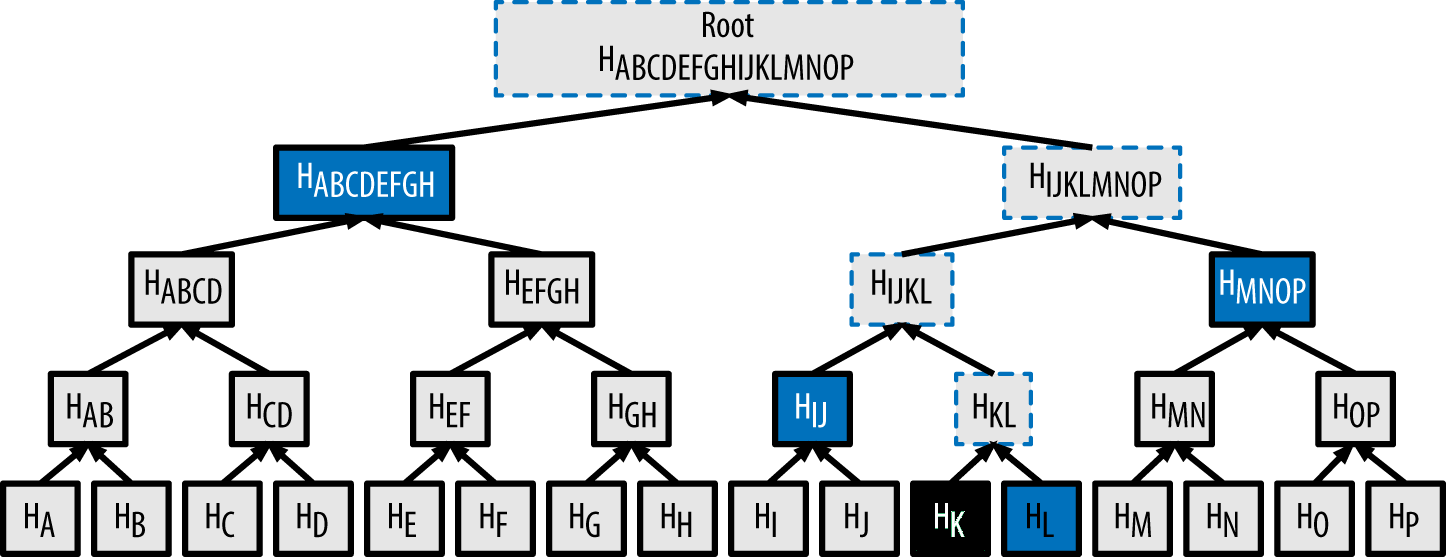
\includegraphics[width=1\linewidth]{img/merkle-tree-path.png}
	\caption{Example of a Merkle path. The path consists of the four hashes with the
  blue background and with these hashes any node can prove that $H_K$ is included
  in the Merkle root by computing four additional pair-wise hashes outlined in a
  dashed line.  }
	\label{fig:Merkle-tree-path}
\end{figure}








%%%%%%%%%%%%%%%%%%%%%%%%%%%
% *** SEVENTH SUB-SECTION ***
%%%%%%%%%%%%%%%%%%%%%%%%%%%
\subsection{The Bitcoin network}

\subsubsection{Network architecture} The Bitcoin network architecture is a
Peer-to-Peer (P2P) network on top of the Internet. P2P means that all the nodes
of the network are peers to each other: they are all equal, there aren't
``special'' nodes, servers, centralized services and heiarchies. The nodes are
interconnected in a mesh network with a ``flat'' topology and the nodes both
provide and consume services at the same time. This architecture, in combination
with a consensus algorithm, is the only one that allows to achieve
decentralization of control. The term ``bitcoin network'' refers to the
collection of nodes running the bitcoin P2P protocol.

Note that, despite the node type, all nodes validate and propagate
transactions/block and discover and maintain connections with peers.

\subsubsection{Node types}

\paragraph{Full nodes} A full node is a node that maintains the full copy of the
blockchain, validates all incoming transactions and blocks and forwards
transactions and blocks to its peers. Since they have a copy of the full ledger,
full nodes can autonomously and authoritatively verify any transaction without
rely on or trust any other system. The ``price'' for this independence however
is that they have to store the full blockchain, which size is currently around
178 GB and increases exponentially \cite{statista}. The Bitcoin Core client
is a full node and in the early years of Bitcoin all nodes were full nodes.

\paragraph{Miners} Miners are nodes that compete to each other to solve the
proof-of-work and create new blocks. Some miners are also full nodes which
maintain a full copy of the blockchain, while others don't and instead they
partecipate to a mining pool which depends on a pool server which maintains a
full copy of the blockchain.

\paragraph{Lightweight clients} Lightweight clients are clients that stores only
a subset of the Bitcoin blockchain and follow a simple payment verification
(SPV) scheme that allows them to verify that a transaction has been included in
the blockchain by receiving and verifying only the block headers relevant to
their wallets (they can't have a picture of all the available UTXOs because they
do not know about all the transactions on the network), without downloading the
block transactions. This kind of clients are designed to run on storage and
power constrained devices such as smartphones, tablets, or embedded systems. In
comparison with a full node: for verifying a transaction a full node checks the
entire chain of blocks for building the UTXO set, a lightweight client instead
basically checks how deep the block that contains the transaction is ``buried''
under other blocks above it. The fact that other nodes accepted the block
containing the transaction and produced more blocks on top of it assures that
the transaction is valid (it's not a double-spend transaction). A lightweight
client checks whether a transaction belong to a block by requesting a
\emph{Merkle path} (see section \ref{sec:Merkle-trees}) which proofs the
belonging and by validating the proof-of-work of the block by computing the hash
of the header.

Note that a transaction can, however, be ``hidden'' from a SPV node because, since
it doesn't have a copy of the ledger with all the transactions, it cannot verify
that a transaction \emph{doesn't exist} (it can only verify that a transaction
\emph{exists}). This vulnerability can be used for example for double spending
the same amount of UTXO by hiding to the node the first transaction. To counter
this vulnerability, SPV nodes connects randomly to several nodes in order to
increase the probability to find at least one honest node.











%%%%%%%%%%%%%%%%%%%%%%%%%%%
% *** EIGHTH SUB-SECTION ***
%%%%%%%%%%%%%%%%%%%%%%%%%%%
\subsection{Mining and Proof of Work} Mining is a resource-intensive
process by which transactions are validated and new blocks are added to the
blockchain. Transactions that become part of a block and added to the blockchain
are considered confirmed, which means that the receivers of the transactions can
spend the value they received.

Roughly one new block is created (\emph{mined}) every 10 minute and Miners after
mining a block are rewarded with two types of rewards: new coins created with
each new block (a basecoin transaction) and transaction fees from all the
transactions included in the block.

\paragraph{Proof of Work} In order to earn the reward, miners compete with each
other to solve a hard problem based on a cryptographic hash algorithm. The
solution to the problem, called the Proof-of-Work, is included in the new mined
block and acts as proof that the miner expended significant computing effort.
The proof of work requirement is given by the following equation:
\begin{equation}\label{eq:proof-of-work}
  H ( N || Prev\_hash || Tx || Tx || . . . Tx) < Target
\end{equation} where H is the SHA256 hash function, N is the nonce
contained in the block header, $Prev\_hash$ is the hash of the previous block,
Tx are the transactions contained in the block, $Target$ is the difficulty
value and $||$ is the concatenate operator.
For example, if the target is $0x10000000000000$ then finding a hash less than
the target means finding a hash that starts with a zero. Consequently, the
difficulty level of the proof of work can be seen as the number of zeros that the
hash of the block has to start with. The only way for finding a valid hash, therefore,
is to use the brute force method, changing the nonce value for every hash
calculation in order to get different hashes until a valid one in found
(any specific hash input to one and only one hash value).
Once the miner met the correct number of zeros, the block is immediately
broadcasted and accepted by other miners.
The difficulty of this work is always adjusted (increased) so as to limit the
rate at which new blocks can be generated by the network to one every 10 minutes.

The algorithm for mining a block can be summarized in the following steps:
\begin{enumerate}
  \item Retrieve the hash of the previous block from the Bitcoin network.
  \item Choose which transaction include in the block (according to their priority).
  \item Compute the double SHA256 hash of the block header (thus in equation
  \ref{eq:proof-of-work} all the transactions $Tx$ are summarized by the root
  of the Merkle tree contained in the block header).
  \item Check whether the resultant hash is lower than the current difficulty level
  (target). If so, then stop the process, otherwise change the nonce (usually it is
  increased by 1) and go back to step 3.
\end{enumerate}















%%%%%%%%%%%%%%%%%%%%%%%%%%%
% *** NINETH SUB-SECTION ***
%%%%%%%%%%%%%%%%%%%%%%%%%%%
\subsection{Consensus} Mining is a key feature of Bitcoin which secures the
bitcoin system and allows to have network-wide consensus without a central
authority. In particular, in Bitcoin consensus is not achieved explicitly since
there is no election or a fixed moment when consensus occurs. Instead, consensus
is an emergent artifact of the asynchronous interaction of thousands of
independent nodes. For this reason, in Bitcoin the consensus process is called
\emph{emergent consensus}. Bitcoin’s decentralized consensus emerges from
four processes that occur independently on nodes across the network:
\begin{itemize}
  \item Independent verification of each transaction by every full node
  \item Independent aggregation of verified transactions into new blocks by mining
  nodes and inclusion of the proof of work
  \item Independent verification of the new blocks by every node and assembly
  into the chain: each node performs a series of tests for validating it before
  propagating it to its peers and inserting it into the blockchain.
  This ensures that only valid blocks are propagated on the network: blocks which
  are tampered with will thus be rejected.
  Thanks to this verification, dishonestly miner (for example miners who write
  themselves a transaction for an arbitrary amount of bitcoin instead of the correct reward have)
  have their blocks rejected and not only lose the reward, but also waste the
  effort expended to find a Proof-of-Work solution.
  \item Independent selection, by every node, of the chain with the most
  cumulative computation demonstrated through Proof-of-Work
\end{itemize}


\paragraph{The 51\% attack} This consensus mechanism is vulnerable to the
so-called 51\% attack, which can be carried out by a group of miners controlling
more than 50\% of the total network hashing power. In this situation the
attackers would be able to prevent new transactions from gaining confirmations,
allowing them to halt payments between some or all users. The attackers would
also be able to reverse transactions that were completed while they were in
control of the network, meaning they could double-spend coins. This attack is
however hypothetical in Bitcoin and even if it was carried out the attacker
wouldn't be able to create new coins or alter old blocks.






















\begin{figure}[b]
	\centering
	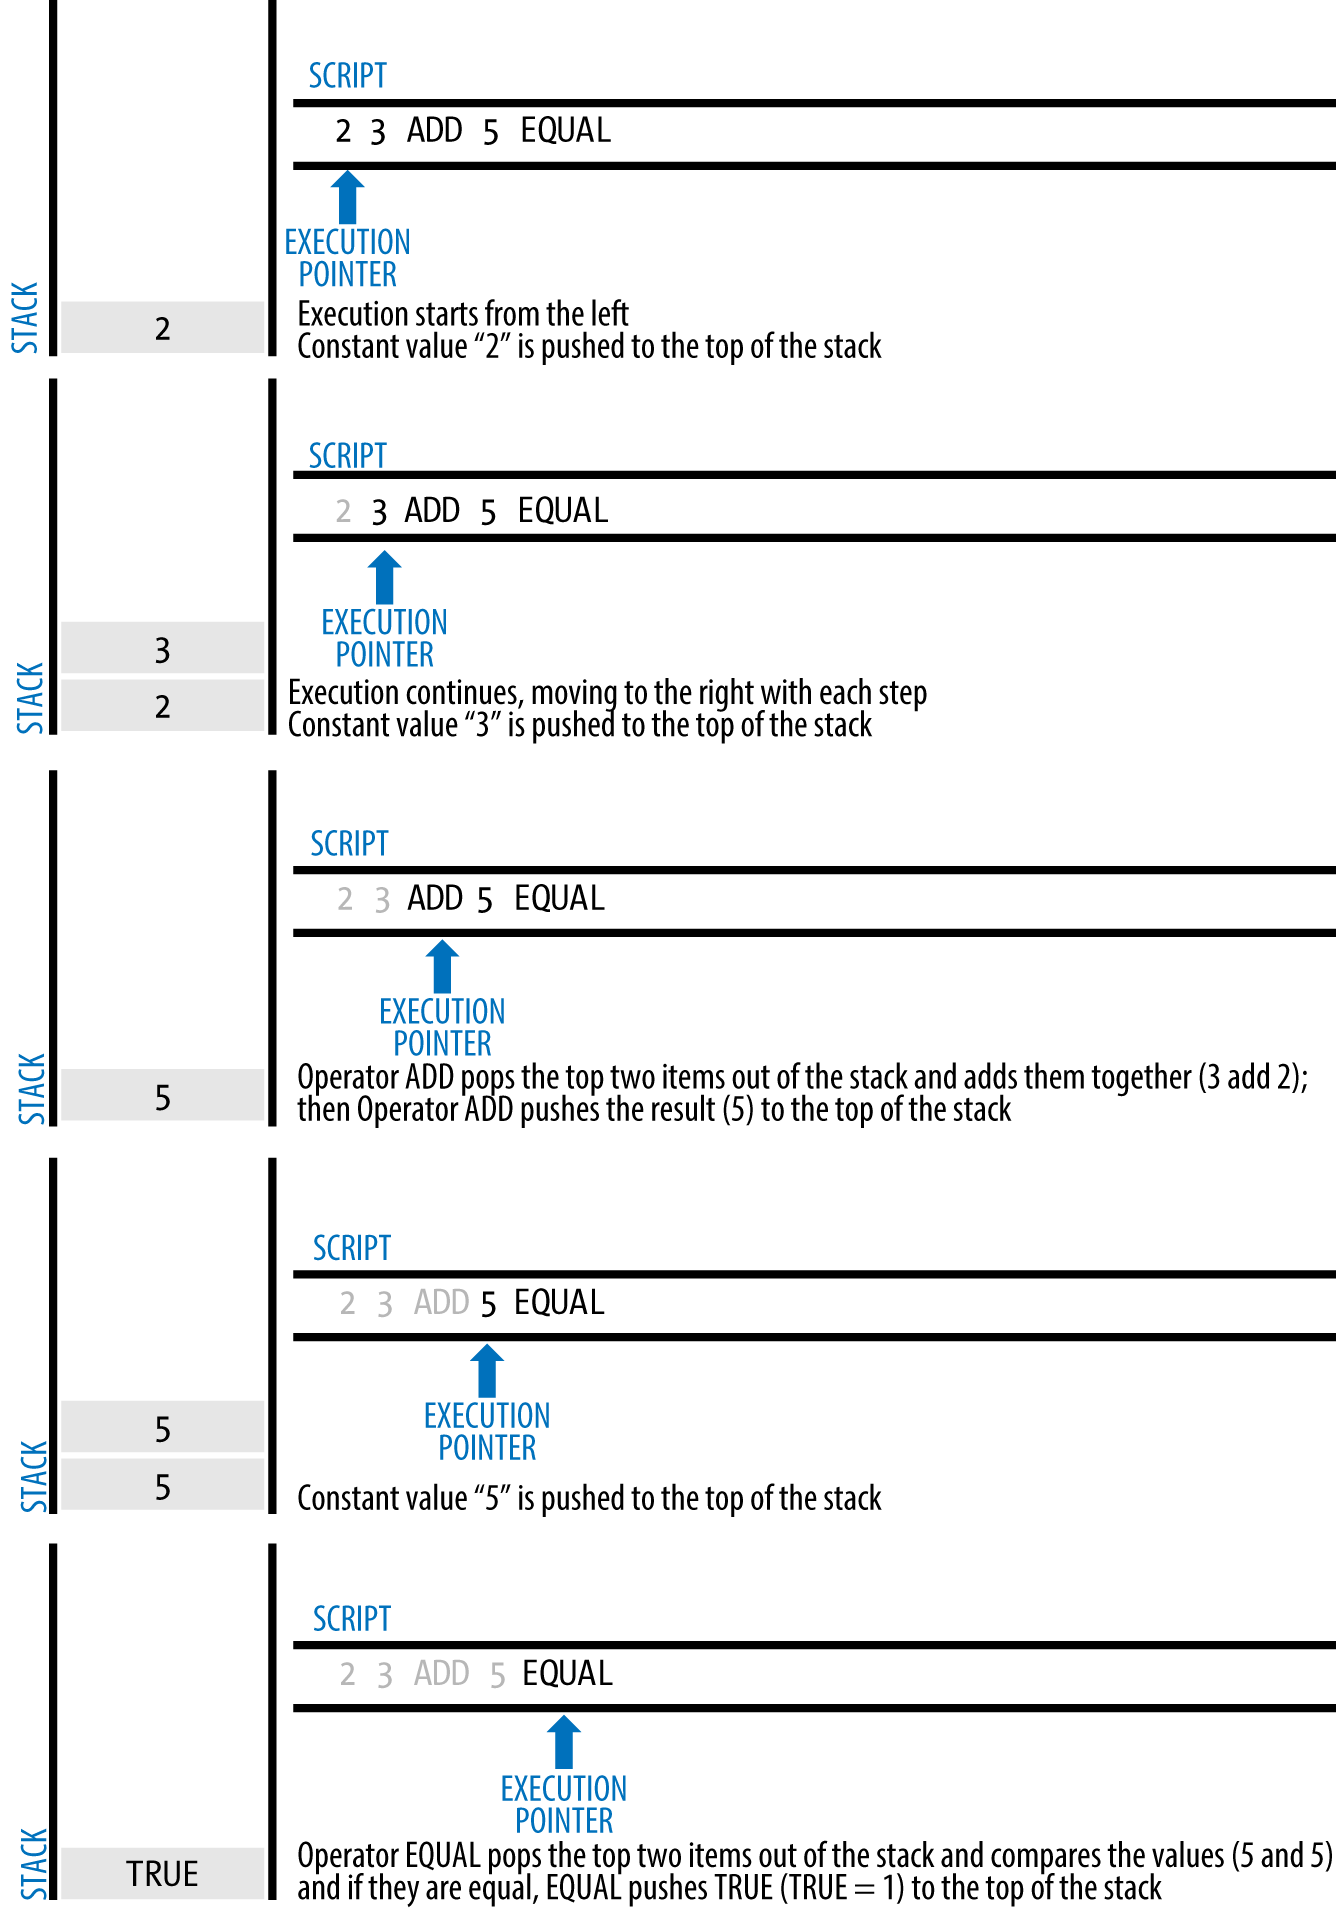
\includegraphics[width=1\linewidth]{img/transaction-script-example.png}
	\caption{Example of a Script program. Image taken from reference \cite{antonopoulos2017mastering}}
	\label{fig:script-example}
\end{figure}
